\documentclass[twocolumn]{article}
\usepackage{graphicx}
\usepackage{amsmath}
\usepackage{siunitx}
\usepackage{fancyhdr} 
\usepackage{fancybox}
\usepackage{float}
\usepackage{listings}
\usepackage[colorlinks=true,linkcolor=black]{hyperref}
%\usepackage[labelformat=empty]{caption}
\usepackage[margin=1.0in]{geometry}

\pagestyle{fancy}

%redefines subsections with letters instesad of numbers
\renewcommand{\thesubsection}{\thesection.\alph{subsection}}

% Center Image Command
\newcommand{\centerimage}[3]{
\begin{figure}[ht!]  
\begin{center}
#1
\caption{#2}
\label{#3}
\end{center}
\end{figure}}

\newcommand{\tstamp}{\today}   
%\renewcommand{\chaptermark}[1]{\markboth{#1}{}}
\renewcommand{\sectionmark}[1]{\markright{#1}}
\lhead[\fancyplain{}{\thepage}]         {\fancyplain{}{Andy Goetz \& Kevin Riedl}}
\chead[\fancyplain{}{}]                 {\fancyplain{}{}}
\rhead[\fancyplain{}{\rightmark}]       {\fancyplain{}{ECE 486 Branch Target Buffer Predictor \& Alpha Predictor}}
\lfoot[\fancyplain{}{}]                 {\fancyplain{\tstamp}{\tstamp}}
\cfoot[\fancyplain{\thepage}{}]         {\fancyplain{}{}}
\rfoot[\fancyplain{\tstamp} {\tstamp}]  {\fancyplain{}{\thepage}}

\author{\LARGE Andy Goetz \& Kevin Riedl}
\date{\today}
\title{\Huge \textbf{ECE 486 Branch Target Buffer \& Alpha Predictor}}

\begin{document}
\maketitle

\section{Abstract}
\section{Acknowledgements}
\section{Background Information}

\section{Implementation Details}
\subsection{Alpha Predictor}
The branch predictor used in this projectwas modeled after
The one described in R. E. Kessler's paper on the Alpha 
21264 processor.
%ADD STUFFS ABOUT ALPHA PREDICTOR CHOICES NOT IN PAPER!!!
\subsection{Implementation Details Not Specified}
%initialization values of the tables
The Alpha paper did not specify a few details about how the predictor
works. The biggest missing piece was the initialization values of the tables.
Over many branches, the values do not matter, but for a small data set given



\subsection{Branch Target Predictor} 

The branch target predictor used in the simulator can be seen in
figure \ref{btbshape}. It is based on a hierarchy of two separate
caches, combined with a return address stack. A small displacement
cache (64 entries by 2 ways) holds entries whose target address is
less than 128 bytes from the program counter. If a target address has
a displacement that is too large to fit in this cache, or an address
is evicted from the displacement cache, it is placed in another,
larger cache that contains direct-mapped addresses. This larger cache
is organized as 64 entries by 8 ways.

\centerimage{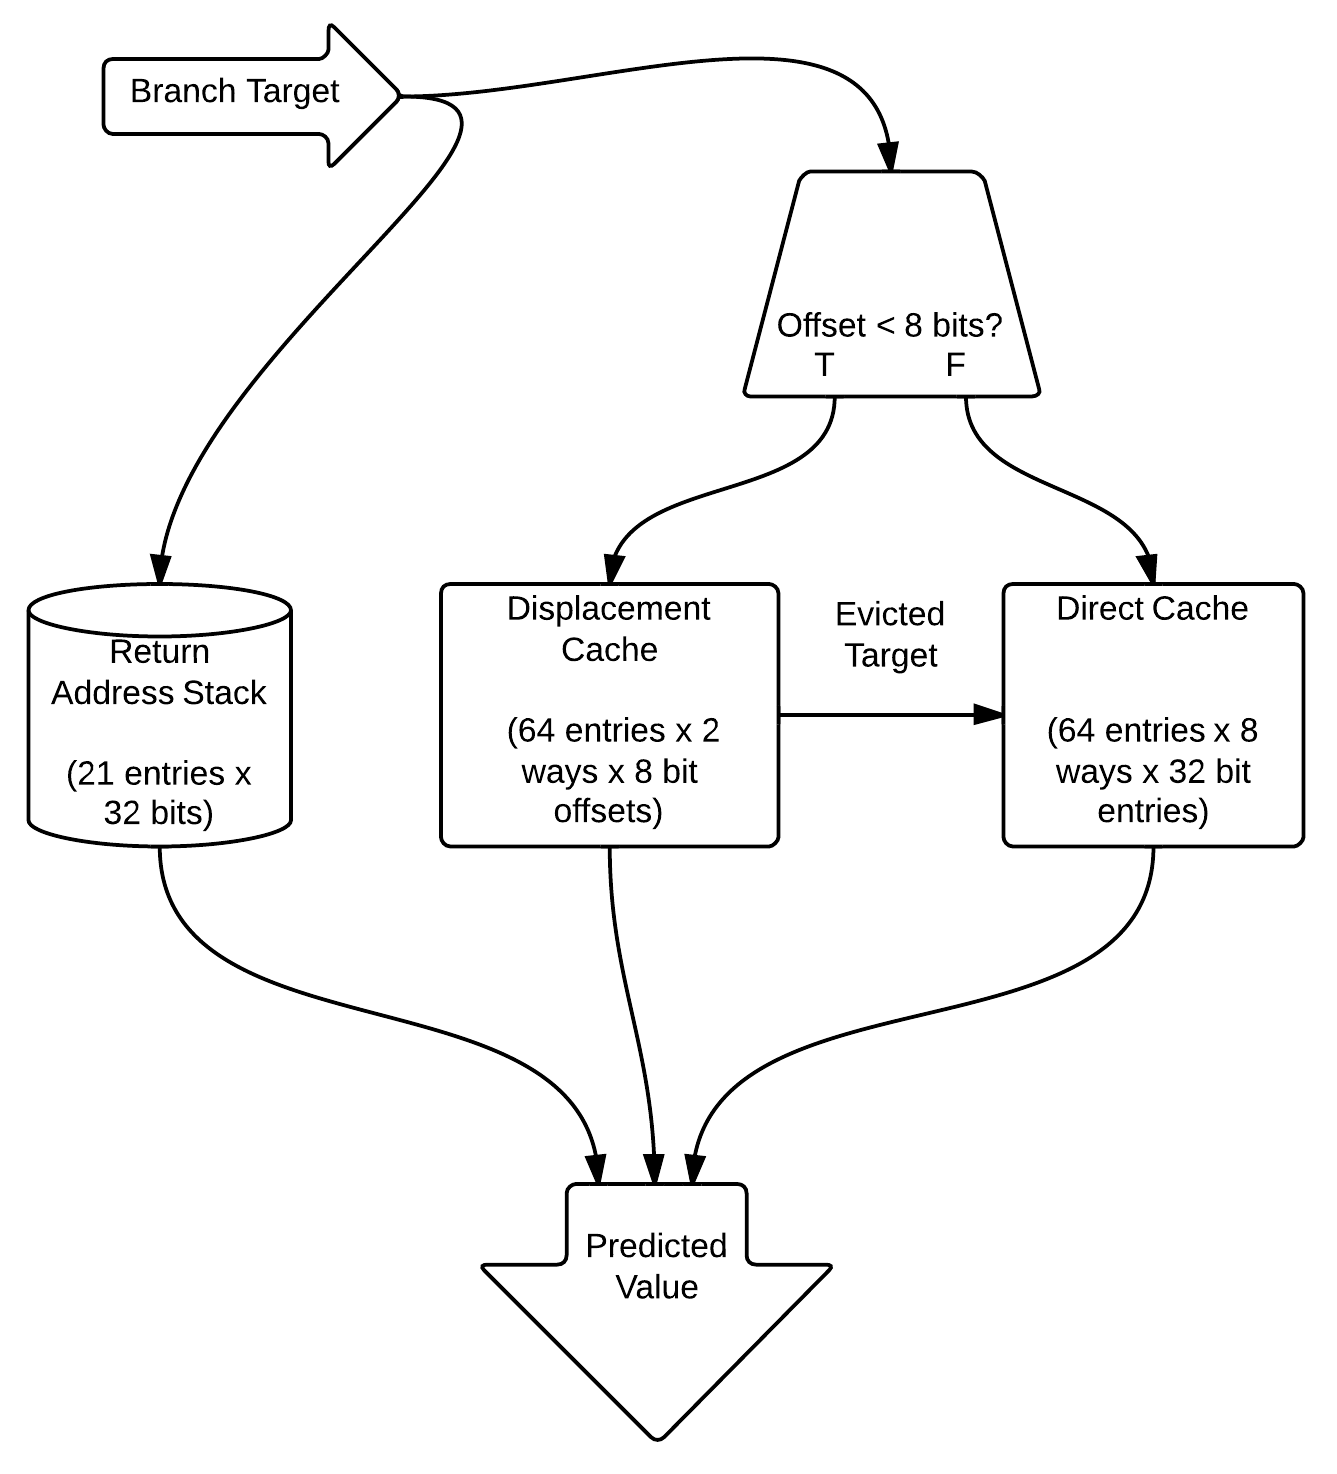
\includegraphics[width=\columnwidth]{BTB.png}}{Branch
  Target Predictor}{btbshape}

The branch target predictor also contains a return address stack. This
stack stores the return address of the last 21 calls. This allows
return addresses to be predicted, regardless of whether or not they
are in the cache. In addition to storing return addresses in the RAS,
return addresses are also placed in the displacement and direct
caches. 

In order to determine the optimal branch predictor design, a generic
predictor framework was designed that used environment variables to
determine the cache hierarchy used by the branch target predictor.
The tunable parameters can be seen in table \ref{envars}. 


\begin{table}
\begin{center}\begin{tabular}{p{.35\columnwidth}p{.5\columnwidth}}
Variable Name & Description \\
\hline
\texttt{BTB\_MAIN\_SIZE} & Index bits of direct cache \\
\texttt{BTB\_MAIN\_WAYS} & Number of ways of direct cache \\
\texttt{BTB\_DISP\_ENTRIES} & Size of entry for displacement cache \\
\texttt{BTB\_DISP\_SIZE} & Index bits of displacement cache \\
\texttt{BTB\_DISP\_WAYS} & Number of ways of displacement cache \\
\texttt{BTB\_WAY\_ALGO} & Way Eviction Policy (LRU or Round Robin) \\
\texttt{BTB\_FUNC\_CAP} & Number of entries in RAS 
\end{tabular}\end{center}
\caption{Kickass}
\label{envars}
\end{table}

In addition, a replacement predictor framework was written using
plaintext tracefiles, allowing for much faster traces, as well as more
detailed predictor statistics.

\section{Testing Methodology}
\centerimage{\includegraphics[width=\columnwidth]{random.pdf}}{Performance of Random Sized BTB Caches}{bgraph}
%Oracle predictor and BTB variables
%Table comparing Faust results to our results for Alpha
\section{Results}
%Table with all prediction rates for all tests
\section{Conclusion}
\newpage
\onecolumn
\section{Predictor.cc}
\lstinputlisting{../predictor.cc}[language=C++, showstringspaces=false]
\end{document}

